\chapter{Introduction}

\section{Object}


The final result that is to be achieved. The object of this template, for example, is to provide guidelines on the structure and content of the core text of a final thesis. 

The main body of the core text of the final thesis and other documents it includes (budget, appendices, terms of reference and/or technical sheets) should be in Times New Roman or Arial, 11 point; the left margin should be 3 cm; the right margin, 2.5 cm; and the top and bottom margins, 2.5 cm. Single spacing should be used.

Students should check the spelling and grammar of all final thesis documents, use the International System of Units (SI) and a consistent number of decimal places, and identify the axes of graphs included in the text.

The length of the core text of the final thesis should not exceed a maximum of 60-70 pages.  

Each table or figure must be numbered and have a title. If a table or figure is from a document consulted by the author, the source must be indicated \cite{eseiaat}.  


\begin{figure}[H]
    \centering
    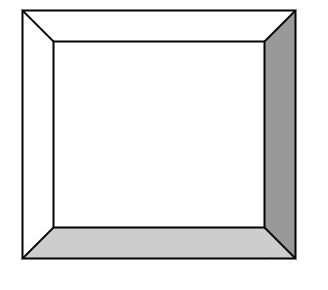
\includegraphics[width=0.3
\linewidth]{Figures/IMATGE_EXEMPLE.jpg}
    \caption{Title of the figure (Source: xxxx)}
    \label{fig:Imatge_exemple}
\end{figure}


\begin{table}[H]

  \centering
   \caption{Title of the table} 
   
  \begin{tabular}{|c|c|c|c|}
    \hline
    \textbf{X} & \textbf{X} & \textbf{X} & \textbf{X} \\
    \hline
    ... & ... & ... & ...\\ \hline
    ... & ... & ... & ...\\ \hline
    ... & ... & ... & ...\\ \hline
    ... & ... & ... & ...\\ \hline
    
  \end{tabular}
  \label{taula_exemple}
 
\end{table}

\section{Scope}

Work packages and deliverables required to arrive at the solution.


\section{Requirements}

Or basic specifications. Limitations of the final solution.

\section{Rationale}

A broad overview of the need for the work, which is then considered from a more specific perspective. The aim is to focus and contextualise the thesis.

